\section{Synchronization and the Sensitivity Gap}
\label{sec:sync}

The decode chain reproduced the article bit-exactly almost immediately;
the measured \emph{sensitivity} did not.  This section documents the
diagnosis --- the most instructive part of the reproduction --- and the
resulting synchronizer.

\subsection{Diagnosis Method}

The tool was a \emph{genie-synchronized} control receiver: the same
demodulator fed the true timing offset and CFO from the channel
simulator.  With genie sync the chain measured $-7.6$\,dB (BPSK
rate-1/3, article channel, PER $\le 10\,\%$)\footnote{All
sensitivities in this report use the article's SNR convention: noise
counted across the full 6\,kHz Nyquist band, of which the signal
occupies $\approx$2.1\,kHz.  Add $\approx$4.5\,dB to compare against
in-band noise only, $\approx$3.8\,dB for the ham 2.5\,kHz
convention.}; the real receiver
initially sat several dB worse.  Every improvement below was validated
by closing part of that gap, and the final residual is $\sim$0.3\,dB
(Section~\ref{sec:results}).

\subsection{Three Defects and Their Fixes}

\paragraph{Preamble power.}  Transmitting the tone combs and ZC symbols
at nominal bin amplitude leaves the preamble region $\sim$7\,dB below
the frame-average power (4 tones versus 23 loaded carriers).  Detection
then fails at SNRs where the payload would decode.  The fix is the
gain scaling of Section~\ref{sec:phy}: $\times\sqrt{5.75}$ on tone
bins and $\times 2$ on ZC bins equalizes per-sample power across the
frame.

\paragraph{Tone-detection metric.}  The article's tone detector
thresholds the in-mask energy \emph{fraction} of a block spectrogram.
That fraction is SNR-dependent --- it fails below $\approx$0\,dB
regardless of threshold --- and divides by zero on noise-free signals.
The implemented metric is a \emph{contrast ratio}: mean in-mask bin
power over mean out-of-mask bin power, evaluated over a grid of
$\pm 4$-bin CFO shifts of the mask, with the denominator regularized
by 1\,\% of the median block power.  The regularizer matters: on clean
signals the out-of-mask power is $\approx$0 and the unregularized
argmax degenerates into a lottery among CFO hypotheses, producing exact
one- and two-bin CFO errors on clean WAV recordings.

\paragraph{Zadoff--Chu time--frequency ambiguity.}  The ZC matched
filter selects the best \emph{normalized} correlation over a search
window after the tone preamble (the raw-peak argmax locks onto the
periodic tiled data symbols).  The subtler defect was scanning the ZC
correlation over $\pm 1$-bin frequency hypotheses: a Zadoff--Chu
sequence's frequency-shifted replica correlates almost as well at a
\emph{shifted time} (the classic ZC time--frequency ambiguity), so at
low SNR the wrong hypothesis wins, injecting a one-subcarrier
(93.75\,Hz) CFO error plus a $\sim$30-sample timing error.  Locking
the composite detector to the zero-CFO hypothesis --- legitimate
because the tone stage already leaves a residual well below half a bin
--- recovered $\approx$1\,dB of sensitivity by itself.

\paragraph{Residual CFO.}  The tone-stage residual CFO is estimated by
a full-length FFT peak over the first tone block (unambiguous over
$\pm 1.5$ bins), refined by a lag-$N$ phase estimate.  A lag-$N$
estimate alone is ambiguous modulo one subcarrier spacing; during
development a lag-16 variant produced 276\,Hz errors because the lag
was not a multiple of the tone-comb period --- the general rule
(enforced in the code) is that a delay-and-correlate lag must be a
multiple of the comb's time-domain period.

\subsection{The STF Preamble Variant}

A commenter on the article proposed replacing the Newman tone comb with
802.11-style short-training tones every 8 bins.  This was implemented
as \texttt{STFOFDMModem}: tone combs on bins $[8,16,24]$ and
$[4,12,20]$ make the tone block periodic with 16 samples, so the
residual CFO comes from a plain Schmidl--Cox-style
delay-and-correlate~\cite{schmidl1997} (lag 16 refined by lag 128),
unambiguous over $\pm 375$\,Hz.  An A/B sweep over the full
$\pm 300$\,Hz CFO range and all eight modulation/rate configurations
shows the two preambles statistically equivalent: identical
$-7.2$\,dB sensitivity, all eight per-configuration sensitivities
within 0.14\,dB, every PER point within $2\sigma$ binomial noise
(Figure~\ref{fig:stf_vs_newman}).  The article-faithful
\texttt{FullOFDMModem} remains the default.

\begin{figure}[H]
    \centering
    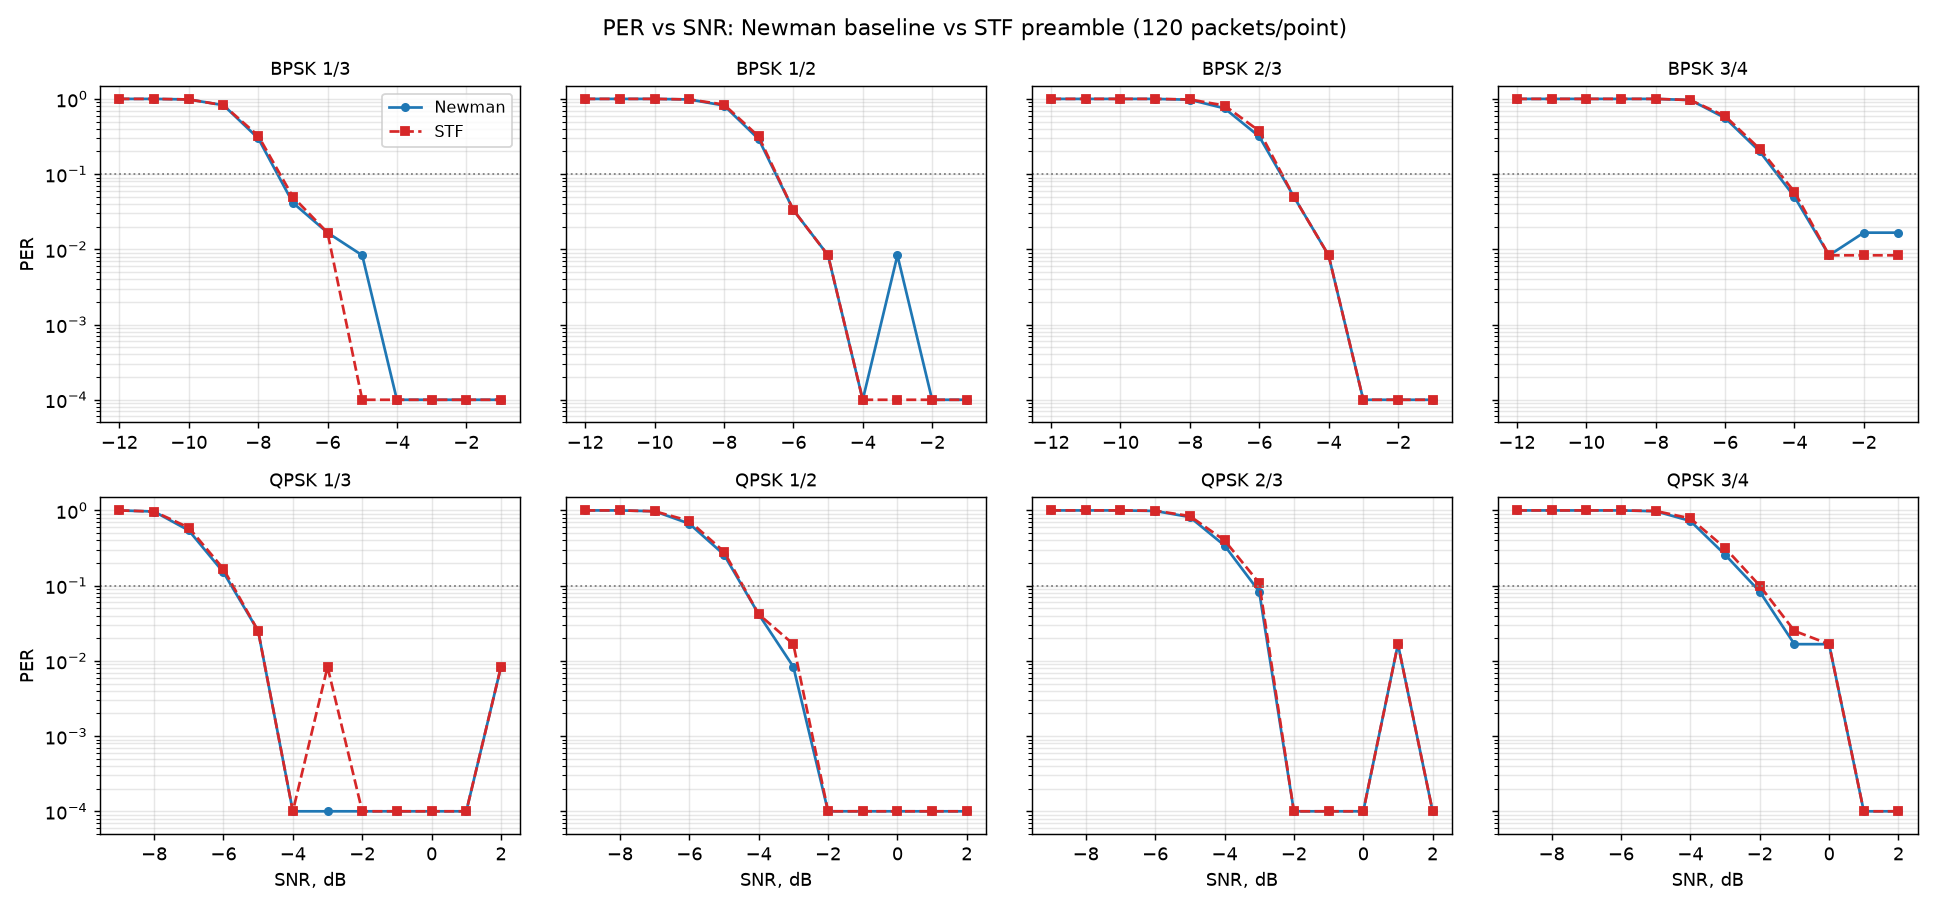
\includegraphics[width=0.9\textwidth]{images/per_stf_vs_newman.png}
    \caption{PER versus SNR for the Newman-tone and STF preamble
             variants over the article channel (same channel
             realizations per arm).}
    \label{fig:stf_vs_newman}
\end{figure}
